\subsection{Rastrigin 1D}

\par Rastrigin is a non-convex function first proposed by Rastrigin as a 2-dimensional function and then generalized later on to multiple dimensions. The one-dimensional version of the function is defined by:

$$
f_3(x) = 10 + x_1^2 - 10 \cos (2 \pi x_1)
$$

It has multiple maxima and minima and its global minima is also at $x=0$.

\par Both functions are tested five times with the Rastrigin 1D function with the same starting random population and a dimensional space of [$-2\pi$, $2\pi$].

\begin{table}[ht]
\scriptsize
\begin{tabular}{l|ccccc}
\textbf{}        & \textbf{Trial 1} & \textbf{Trial 2} & \textbf{Trial 3} & \textbf{Trial 4} & \textbf{Trial 5} \\
\hline
LOA End Fitness  & 3.2384E-09       & 2.4366E-09       & 2.7632E-08       & 3.3077E-08       & 2.8756E-08       \\
LOA Evaluations  & 3401             & 3296             & 3442             & 3423             & 3379             \\
iLOA End Fitness & 1.7764E-15       & 3.5527E-15       & 3.6447E-09       & 2.2848E-10       & 2.8727E-11       \\
iLOA Evaluations & 2559             & 2631             & 2664             & 2694             & 2919
\end{tabular}
\caption{ \scriptsize LOA vs. iLOA: Rastrigin 1D ($f_3$)}
\end{table}

\begin{figure}
  \centering
  \begin{subfigure}[b]{0.4\textwidth}
    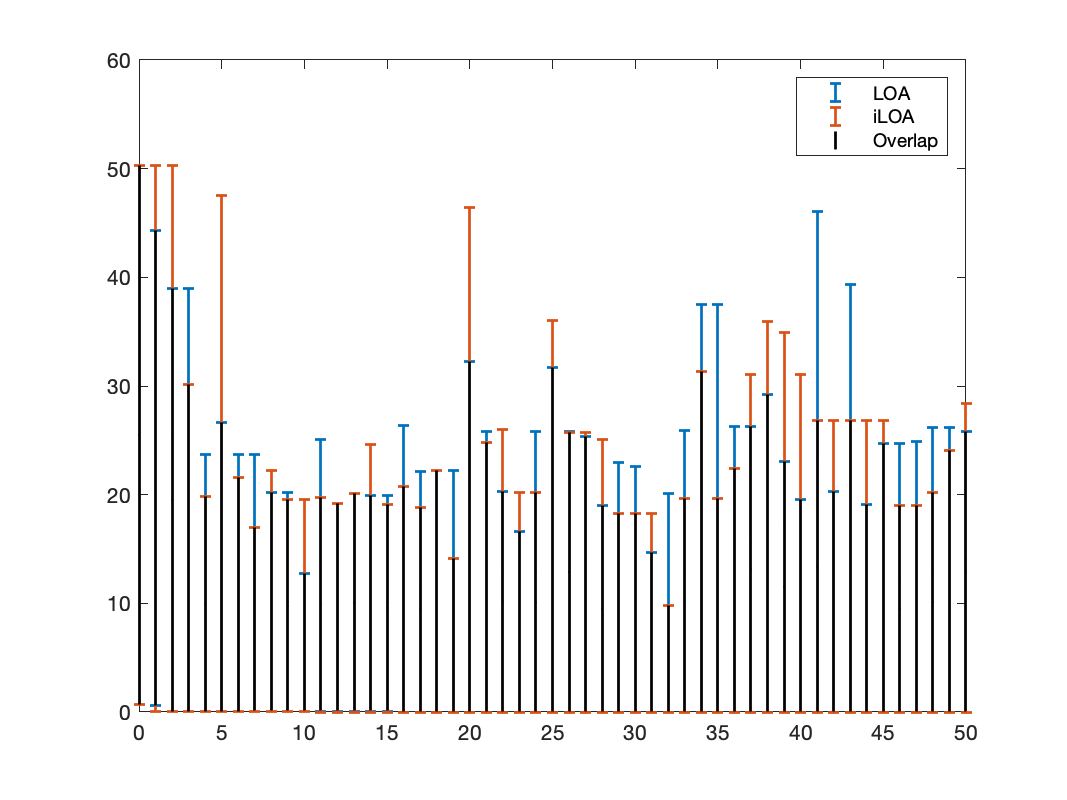
\includegraphics[width=\textwidth]{img/bars/f3/1}
    \caption{ \scriptsize Trial 1: Fitness Range (y) over Iterations (x)}
    \label{fig:f3-b-1}
  \end{subfigure}
  \begin{subfigure}[b]{0.4\textwidth}
    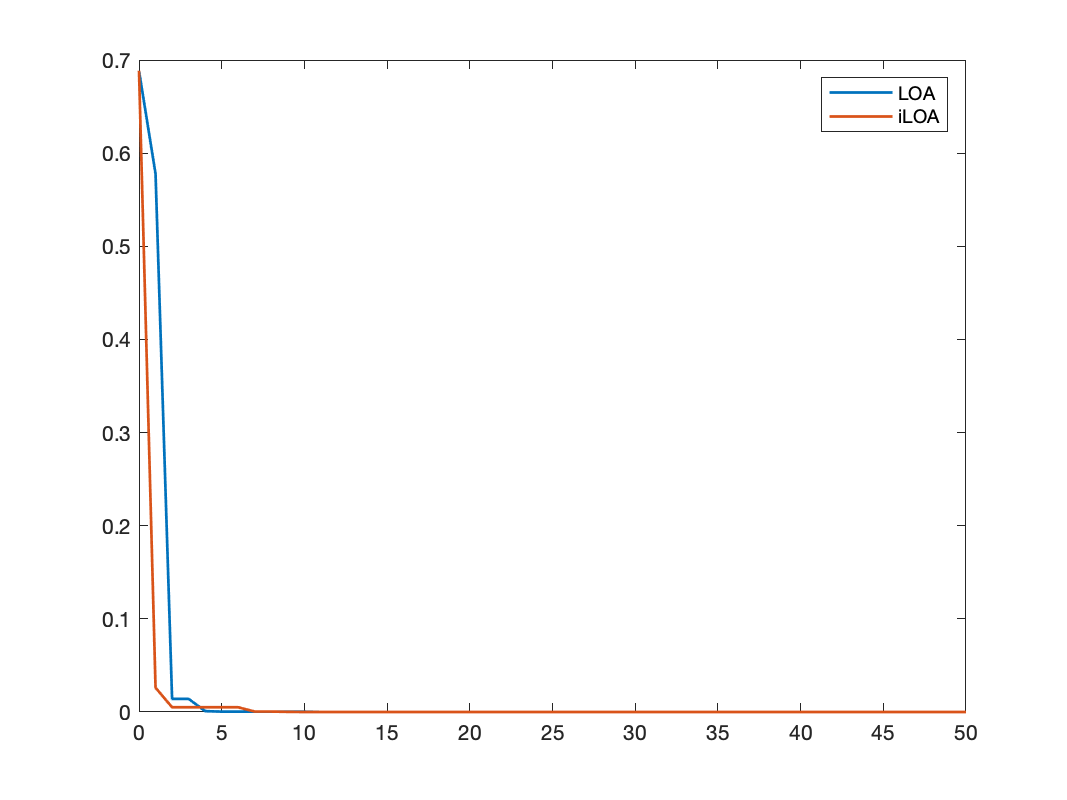
\includegraphics[width=\textwidth]{img/fits/f3/1}
    \caption{ \scriptsize Trial 1: Minimum Fitness (y) over Iterations (x)}
    \label{fig:f3-f-1}
  \end{subfigure}

  \begin{subfigure}[b]{0.4\textwidth}
    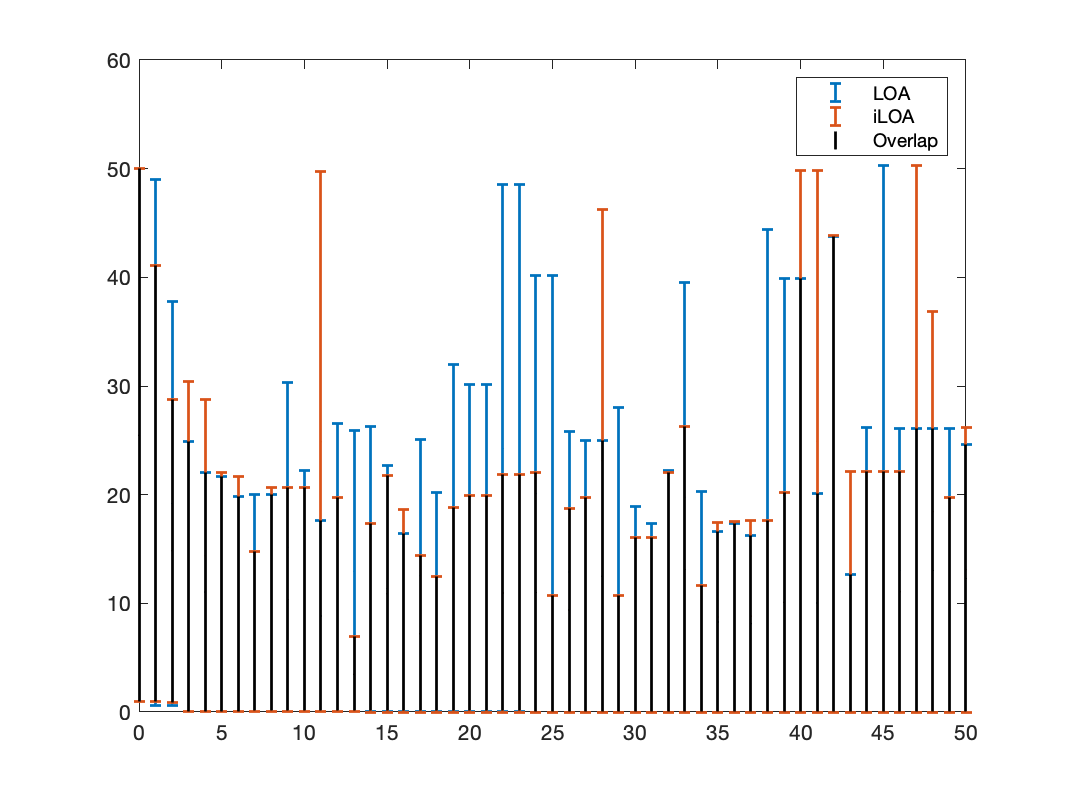
\includegraphics[width=\textwidth]{img/bars/f3/2}
    \caption{ \scriptsize Trial 2: Fitness Range (y) over Iterations (x)}
    \label{fig:f3-b-2}
  \end{subfigure}
  \begin{subfigure}[b]{0.4\textwidth}
    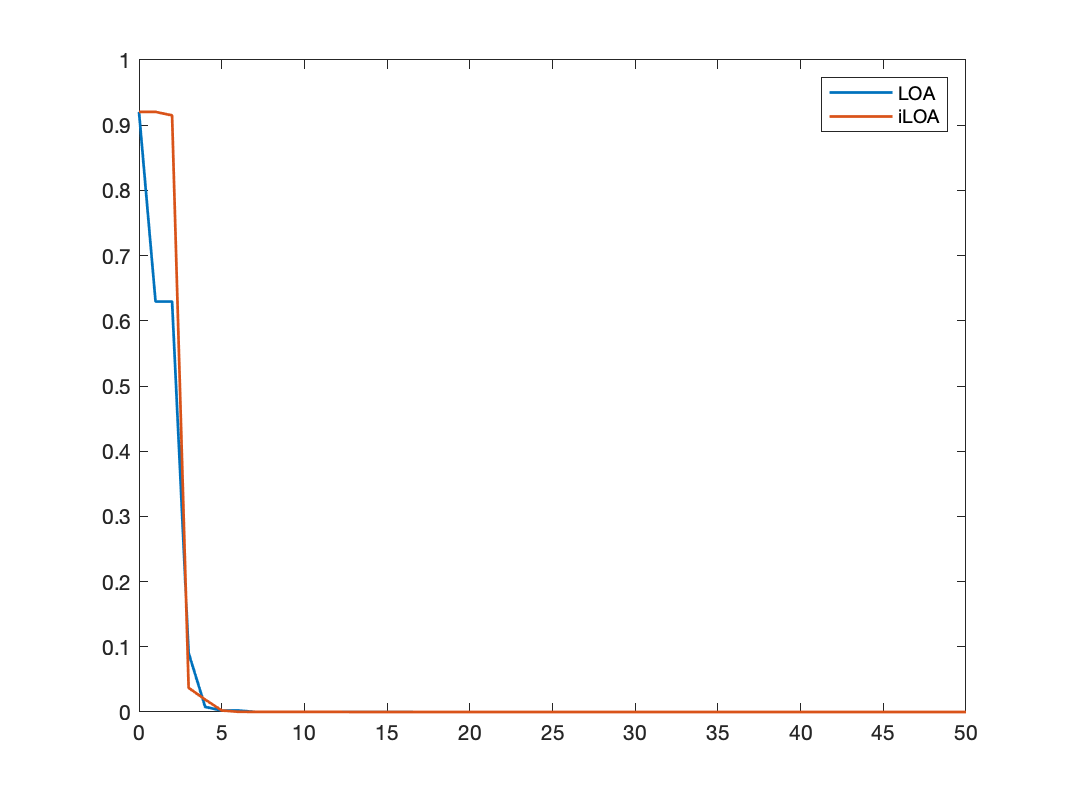
\includegraphics[width=\textwidth]{img/fits/f3/2}
    \caption{ \scriptsize Trial 2: Minimum Fitness (y) over Iterations (x)}
    \label{fig:f3-f-2}
  \end{subfigure}

  \begin{subfigure}[b]{0.4\textwidth}
    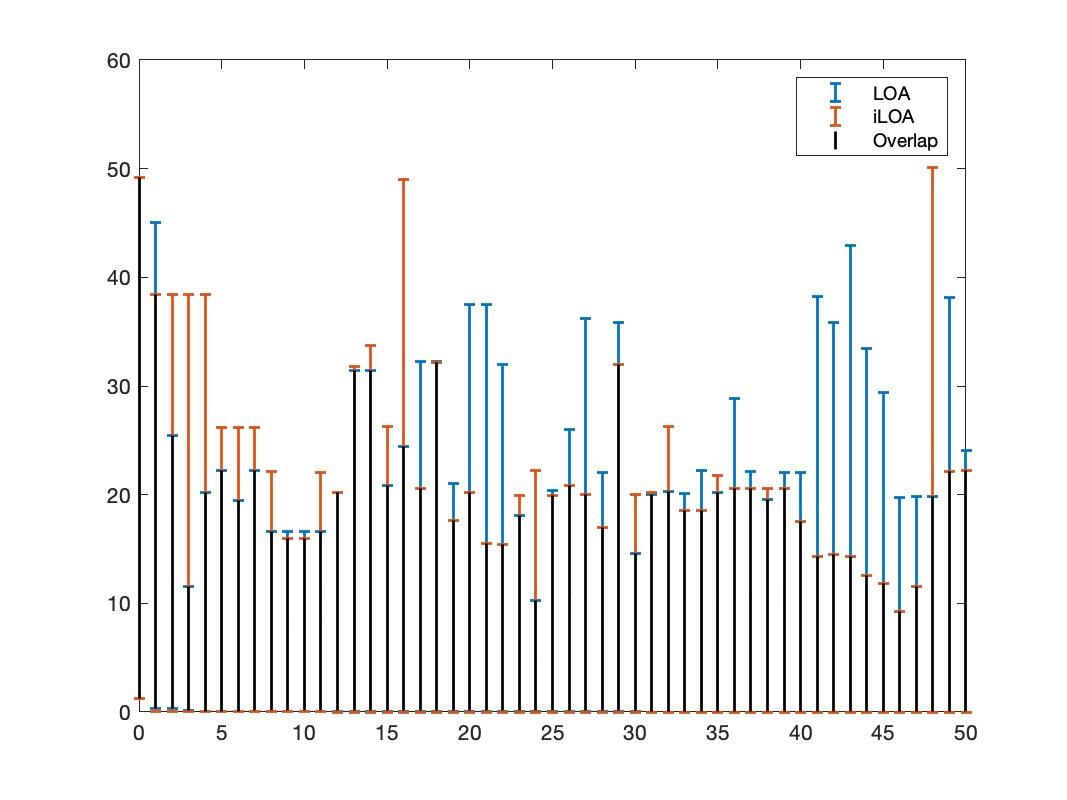
\includegraphics[width=\textwidth]{img/bars/f3/3}
    \caption{ \scriptsize Trial 3: Fitness Range (y) over Iterations (x)}
    \label{fig:f3-b-3}
  \end{subfigure}
  \begin{subfigure}[b]{0.4\textwidth}
    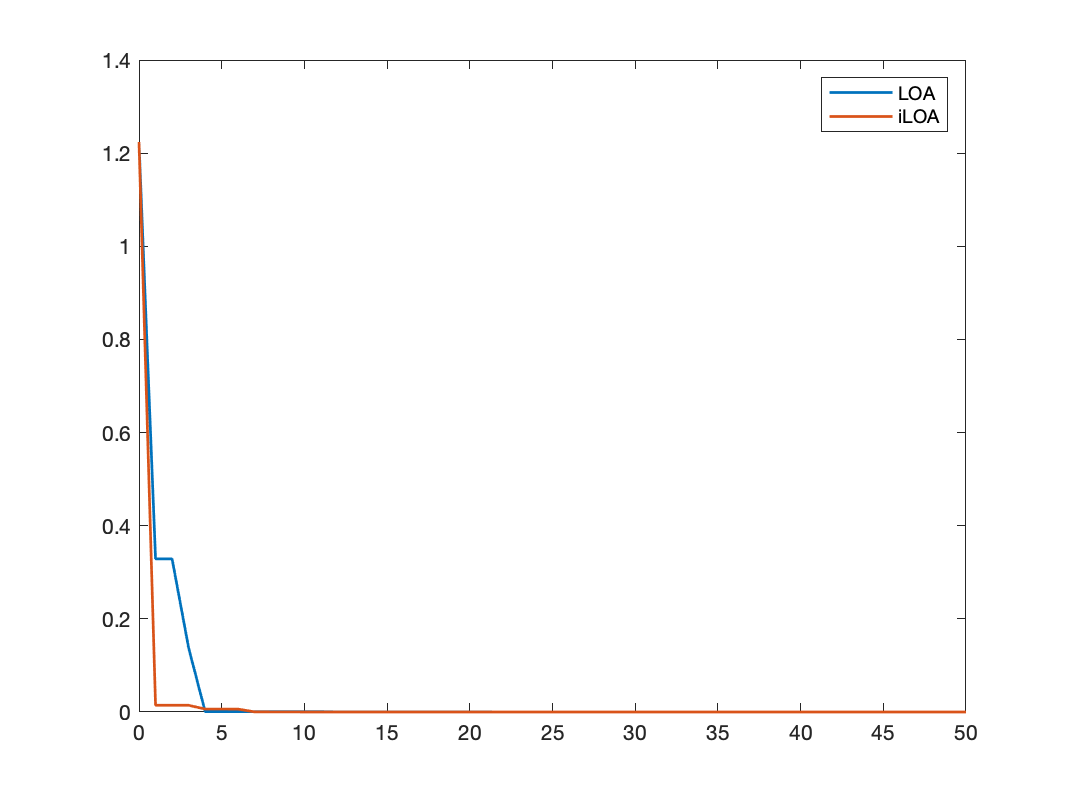
\includegraphics[width=\textwidth]{img/fits/f3/3}
    \caption{ \scriptsize Trial 3: Minimum Fitness (y) over Iterations (x)}
    \label{fig:f3-f-3}
  \end{subfigure}

  \begin{subfigure}[b]{0.4\textwidth}
    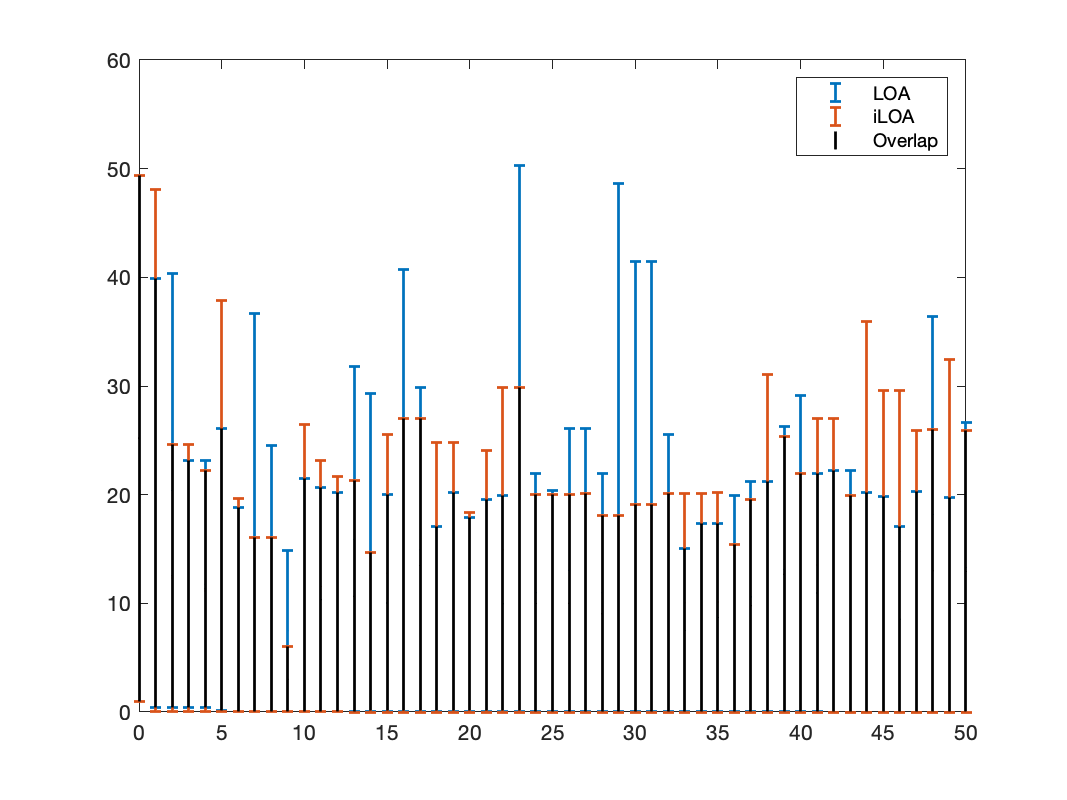
\includegraphics[width=\textwidth]{img/bars/f3/4}
    \caption{ \scriptsize Trial 4: Fitness Range (y) over Iterations (x)}
    \label{fig:f3-b-4}
  \end{subfigure}
  \begin{subfigure}[b]{0.4\textwidth}
    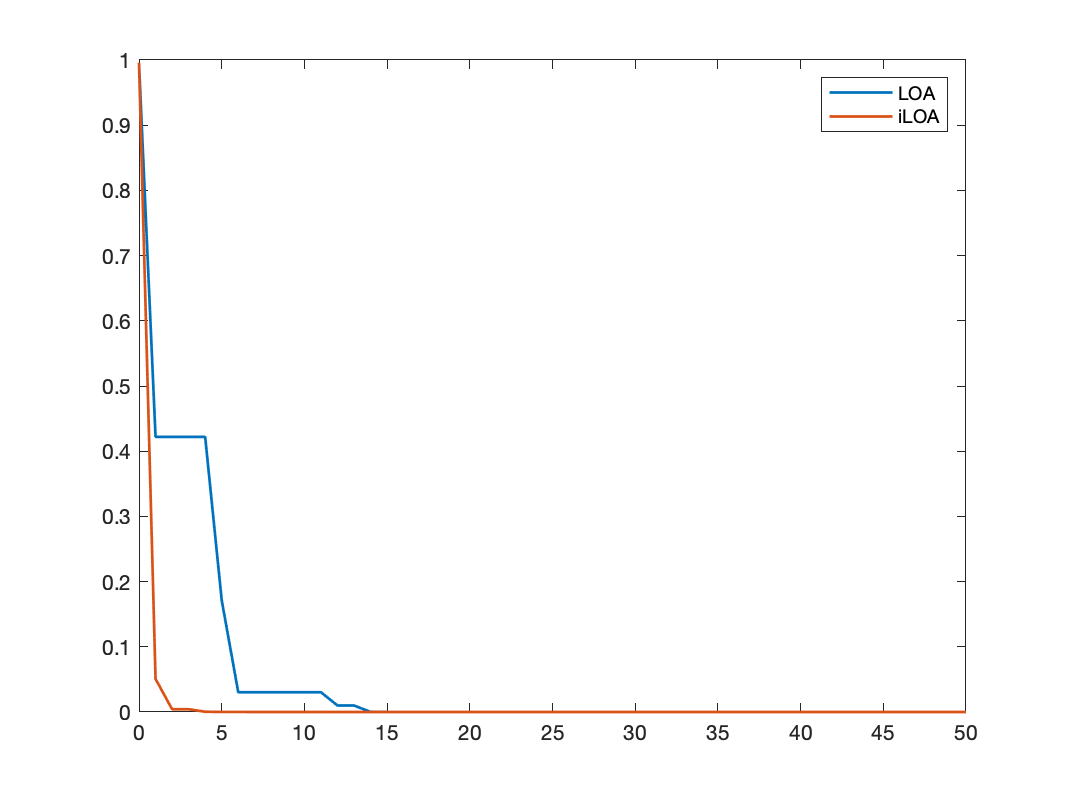
\includegraphics[width=\textwidth]{img/fits/f3/4}
    \caption{ \scriptsize Trial 4: Minimum Fitness (y) over Iterations (x)}
    \label{fig:f3-f-4}
  \end{subfigure}

  \begin{subfigure}[b]{0.4\textwidth}
    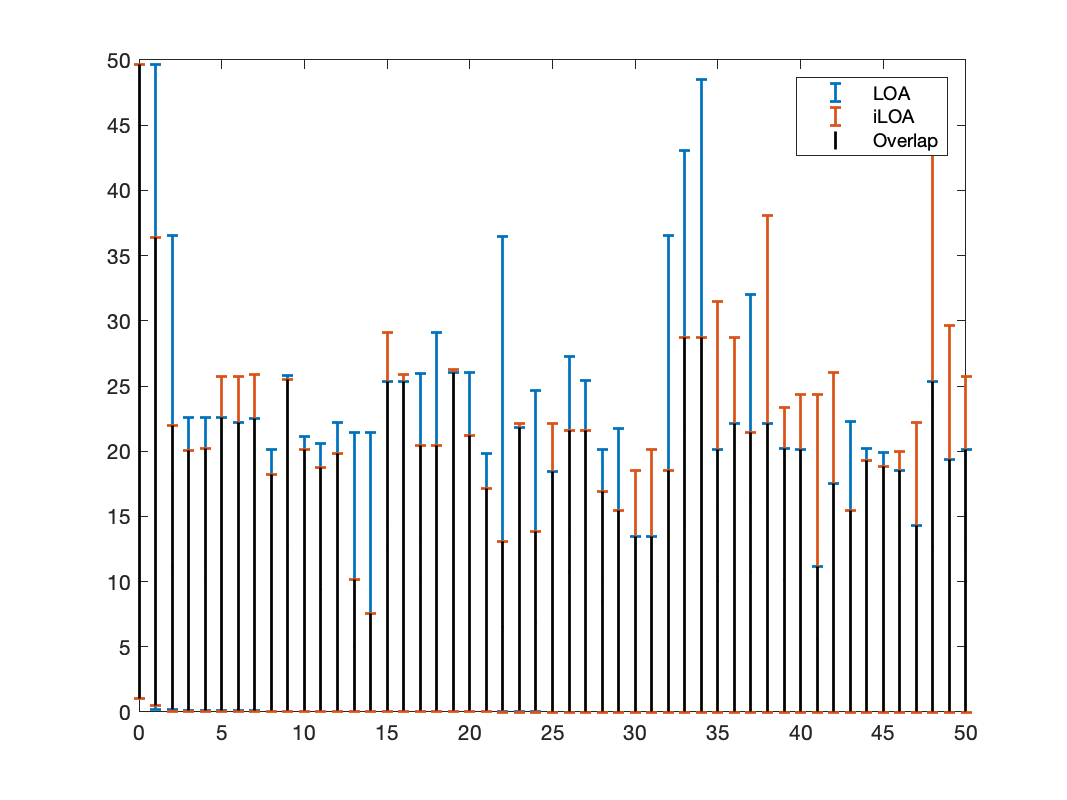
\includegraphics[width=\textwidth]{img/bars/f3/5}
    \caption{ \scriptsize Trial 5: Fitness Range (y) over Iterations (x)}
    \label{fig:f3-b-5}
  \end{subfigure}
  \begin{subfigure}[b]{0.4\textwidth}
    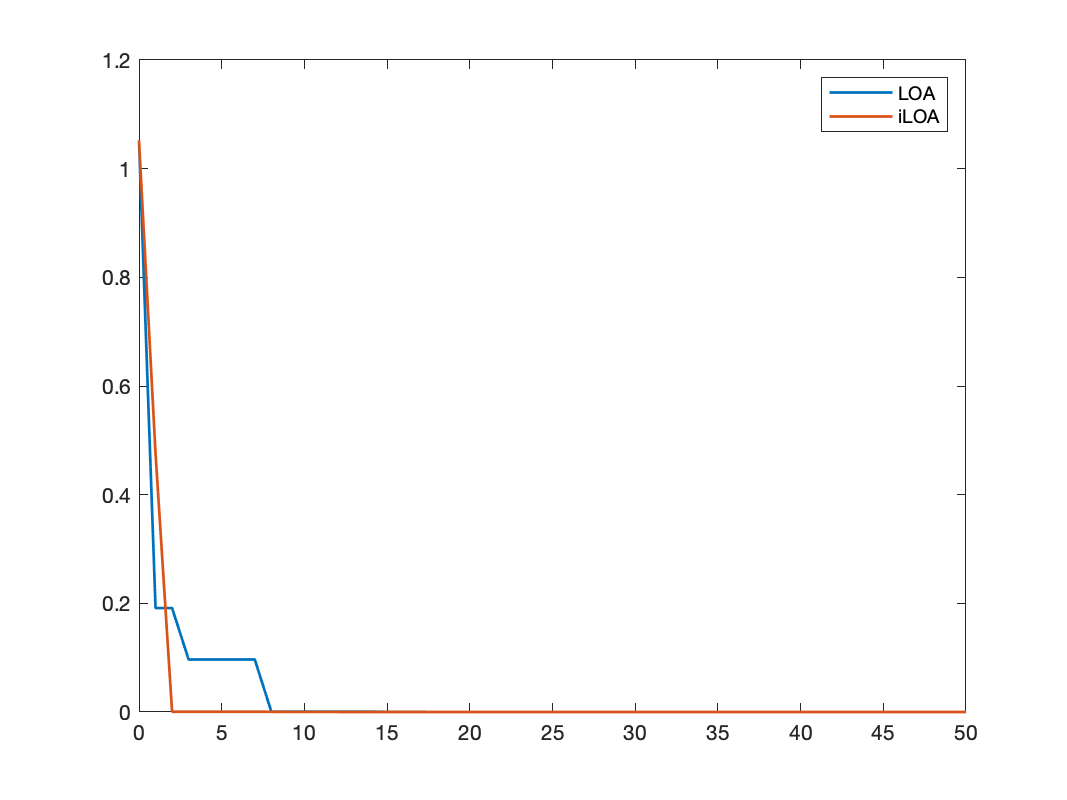
\includegraphics[width=\textwidth]{img/fits/f3/5}
    \caption{ \scriptsize Trial 5: Minimum Fitness (y) over Iterations (x)}
    \label{fig:f3-f-5}
  \end{subfigure}

  \caption{ \scriptsize LOA vs. iLOA: Rastrigin 1D ($f_3$)}
\end{figure}
